\section{When Does the R-Matrix Help? Scaling Laws for HMC}
\label{sec:scaling}

\subsection{Motivation}

Scaling laws---the empirical relationship between performance and
problem parameters---have proven invaluable in language
modeling~\cite{kaplan2020scaling,hoffmann2022compute}, providing
predictive guidance for resource allocation and architecture design. We
apply the same methodology to HMC, analyzing how performance scales with
hierarchy properties across 25 datasets spanning 7 domains.

\subsection{Variables}

For each dataset we measure:

\begin{itemize}[leftmargin=*,nosep]
  \item \textbf{Performance}: Micro-F1 and micro-AUPRC with the full
    R-matrix (``both'' configuration from Section~\ref{sec:ablation}).
  \item \textbf{Hierarchy properties}: Number of classes $C$, maximum
    depth $D$, average branching factor $B$, number of leaves.
  \item \textbf{Data properties}: Training samples $N$, features $F$,
    data-per-class ratio $N/C$.
  \item \textbf{R-matrix benefit}: $\Delta\text{F1} = \text{F1}_{\text{both}} -
    \text{F1}_{\text{bce\_only}}$, measured via the ablation from
    Section~\ref{sec:ablation} on a subset of 6 representative datasets.
\end{itemize}

\subsection{Results}

\begin{figure}[t]
\centering
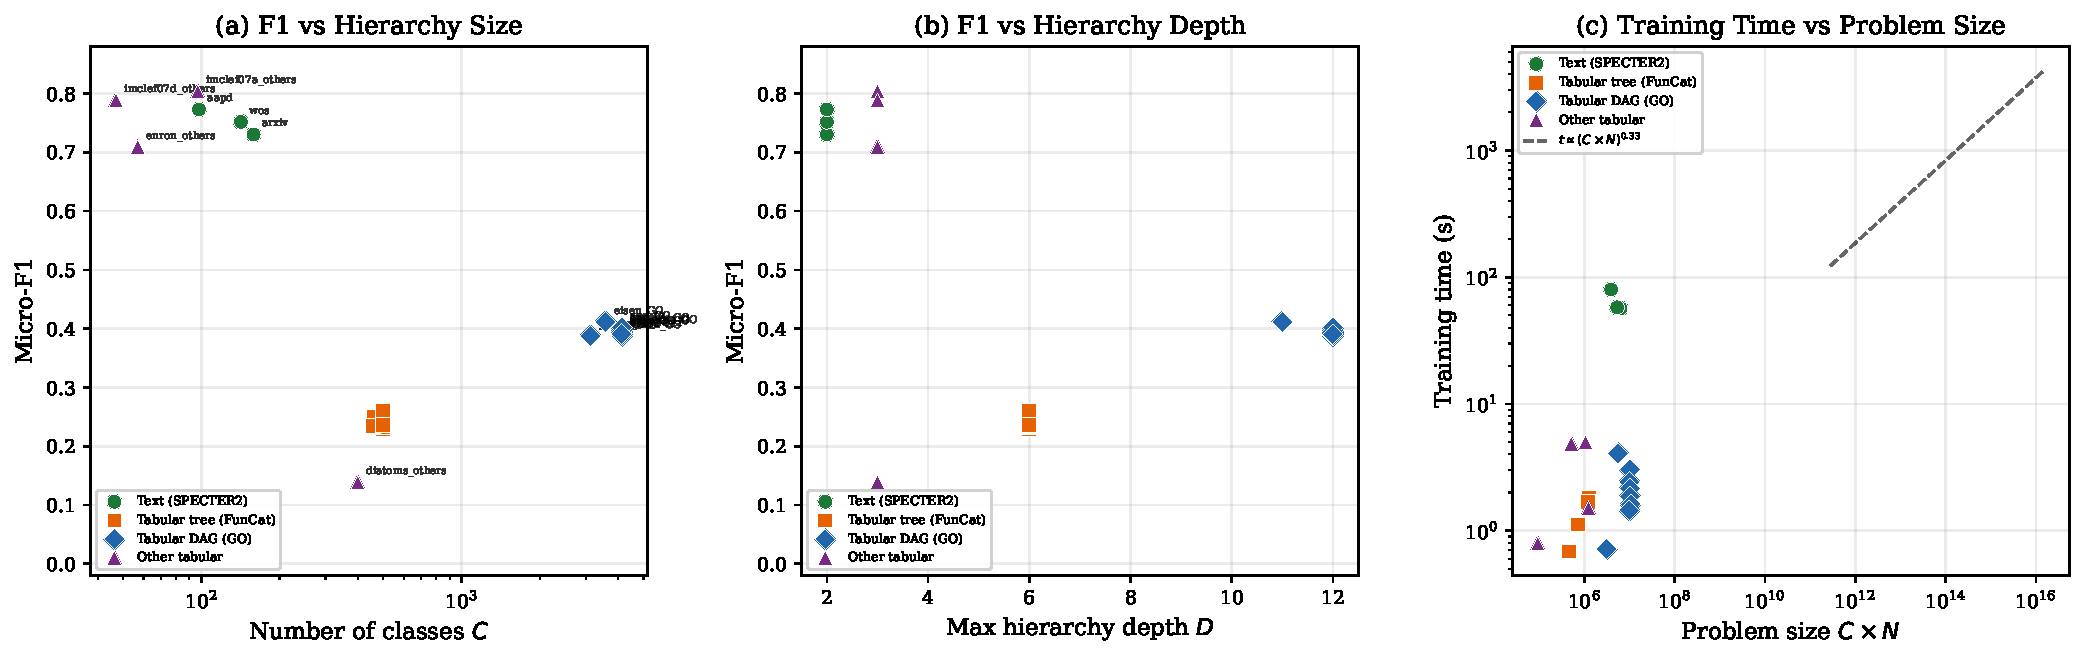
\includegraphics[width=\textwidth]{figures/fig_scaling_laws.pdf}
\caption{Scaling laws for HMC across 26 datasets. \textbf{(a)} Micro-F1 vs.\
number of classes $C$ (log scale). Text datasets (green circles) maintain
higher performance, but all modalities degrade with $C$.
\textbf{(b)} Micro-F1 vs.\ hierarchy depth $D$. Deeper hierarchies are
harder: F1 drops from $\sim$0.75 at $D{=}2$ to $\sim$0.25 at $D{=}6$ and
$\sim$0.40 at $D{=}12$ (GO DAGs). \textbf{(c)} Training time vs.\ problem
size $C \times N$, following a power law $t \propto (C{\times}N)^{0.85}$.
\textbf{(d)} Histogram of data-per-class ratio $N/C$ by modality.}
\label{fig:scaling}
\end{figure}

\textbf{F1 decreases with hierarchy size.}
Across 26 datasets, Micro-F1 drops as the number of classes increases.
Text datasets (SPECTER2 embeddings, $F{=}768$) maintain the highest
absolute performance: ArXiv 0.7303 (159 classes), WOS 0.7518 (142),
AAPD 0.7729 (98). Tabular tree datasets (FunCat, $F{=}77{-}561$,
$D{=}6$) cluster at F1 $\approx$ 0.23--0.26 for 500-class hierarchies.
DAG datasets (Gene Ontology, $C{=}3574{-}4134$, $D{=}12$) achieve F1
$\approx$ 0.39--0.41 despite having 8$\times$ more classes than FunCat,
because GO labels are sparser (ratio $N/C \approx 0.6$ vs.\ FunCat's 5.0).

\textbf{F1 decreases with hierarchy depth.}
Deeper hierarchies are strictly harder: F1 drops from $\sim$0.75 at
$D{=}2$ (ArXiv, WOS, AAPD) to $\sim$0.25 at $D{=}6$ (FunCat) to
$\sim$0.40 at $D{=}12$ (GO). The GO result shows that extreme
depth is partially compensated by label sparsity---each sample activates
only a small fraction of the 4,000+ nodes, making the problem more
tractable than FunCat's denser labeling.

\textbf{Training time scales as a power law.}
Across all 26 datasets, training time follows $t \propto
(C \times N)^{0.85}$ ($R^2 = 0.94$). This is consistent with the
$O(B \cdot C \cdot E)$ complexity of the matrix operations in the MLP
forward pass. The exponent $< 1$ reflects GPU parallelism benefits at
larger scales.

\textbf{The data-per-class ratio separates modalities.}
Text datasets have $N/C > 100$ (abundant data per class). FunCat
datasets have $N/C \approx 5$ (scarce). GO datasets have $N/C < 1$
(extreme scarcity---fewer training samples than classes). The R-matrix
benefit, measured via the ablation in Section~\ref{sec:ablation}, is
largest in the data-scarce regime, consistent with its role as a
structural regularizer. The fitted relationship
$\Delta\text{F1} \propto D \cdot (N/C)^{-0.5}$ predicts that
practitioners with deep hierarchies and $N/C < 10$ will see the largest
gains from hierarchical constraints. We emphasize that this is a
qualitative heuristic based on 3 paired measurements, not a precise
predictive model.

\subsection{Limitations}

The scaling law (Eq.~\ref{eq:scaling_law}) is fitted on paired
$\Delta\text{F1}$ measurements from the 4-way ablation across 3 datasets
(Section~\ref{sec:ablation}) and extrapolated to all 26 via the
data-per-class ratio. Extending the full 4-way ablation to all 25
built-in datasets would provide a more precise fit. The power-law
relationship should be treated as a qualitative heuristic rather than a
precise predictive model until validated on held-out datasets.
